\chapter{Architecture}
\label{chp:architecture} 

The purpose of this thesis is to build an end to end system, to be able to transfer data all the way from a sensor connected to a microcontroller to a server. This chapter will describe in detail how the different components of the system has been connected together, and how the different protocols has been configured to read and transfer data efficiently. 


\begin{figure}[h]
    \centering
    \includegraphics[scale=0.7]{MasterArchitecture.png}    \caption{System architecture}
    \label{fig:systemArchitecture}
\end{figure}

\newpage

There are two main limitations in a network such as this:

\begin{itemize}
  \item Computational power in the different nodes 
  \item Network limitations between the nodes
\end{itemize}

A central part of the testing in this thesis will be to test the different limitations, and to understand the pros and cons of doing computations in end nodes, compared to transferring information to a server with \textit{much} more computational power. Power usage is very often closely related to computational power, and will also be a central factor. The next section will contain a walk through of the system, from the smallest to the biggest component, to explain their computational and power capabilities, and how they can communicate efficiently. 

%Computational power is closely related to power usage. The nRF52 microcontroller is battery powered using a small \textit{3V Lithium CR 2032} battery. Given this limitation the computational power will be limited as well. The optimal solutions therefore seems to handle as little data as possible here. 


%Figure \ref{fig:systemArchitecture} shows how the complete End-to-End system of this thesis is set up. In short terms, the \textit{ADXL345 Accelerometer} is connected to a \textit{Nordic Semiconductor nRF52} using the \gls{i2c} interface. This requires four cables (noted from nRF52 to ADXL345): 

\section{Connecting nRF52 and ADXL345}

The ADXL345 Accelerometer used was connected using \gls{i2c}, which is quite straight forward using the nRF52. Connection scheme is as follows (nRF52 -> ADXL345): 

\begin{itemize}
  \item 5V -- VIN			\textit{Power source}
  \item GND -- GND 			\textit{Ground}
  \item P0.27 -- SDA		\textit{\gls{i2c} SDA}
  \item P0.26 -- SCL		\textit{\gls{i2c} SCL}
\end{itemize} 




\begin{figure}[h]
    \centering
    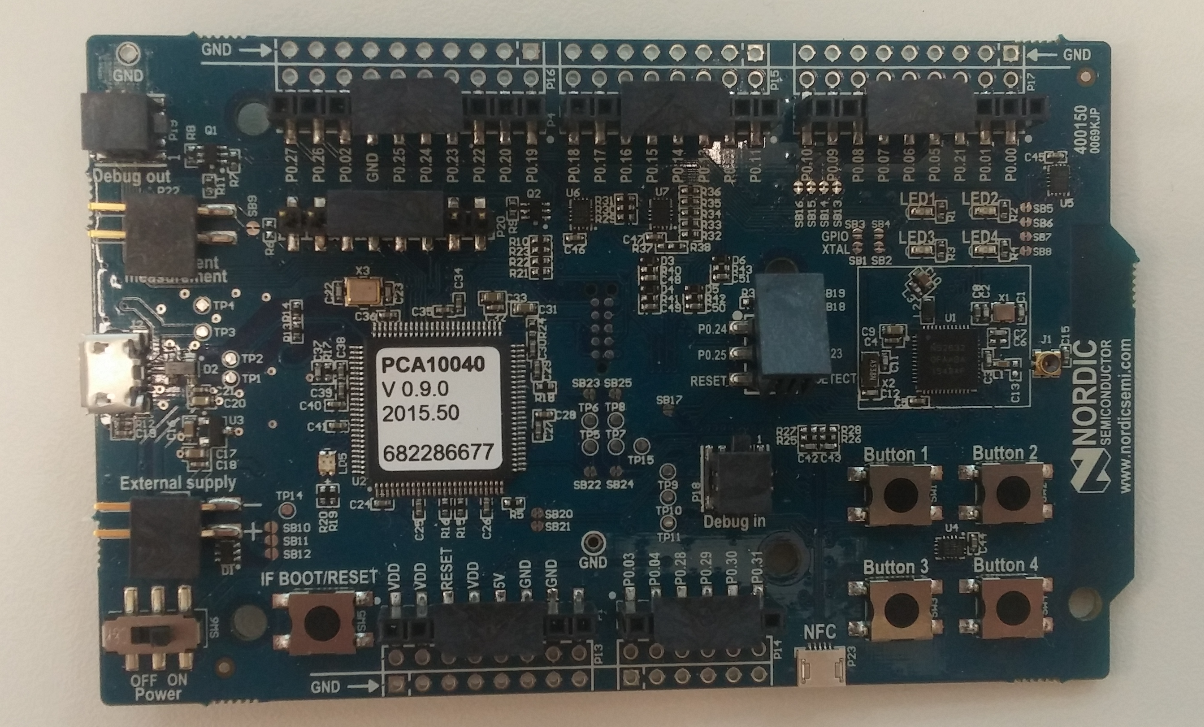
\includegraphics[scale=0.32]{nrf52.png}    \caption{Nordic Semiconductor NRF52}
    \label{fig:adxl345}
\end{figure}

\begin{figure}[h]
    \centering
    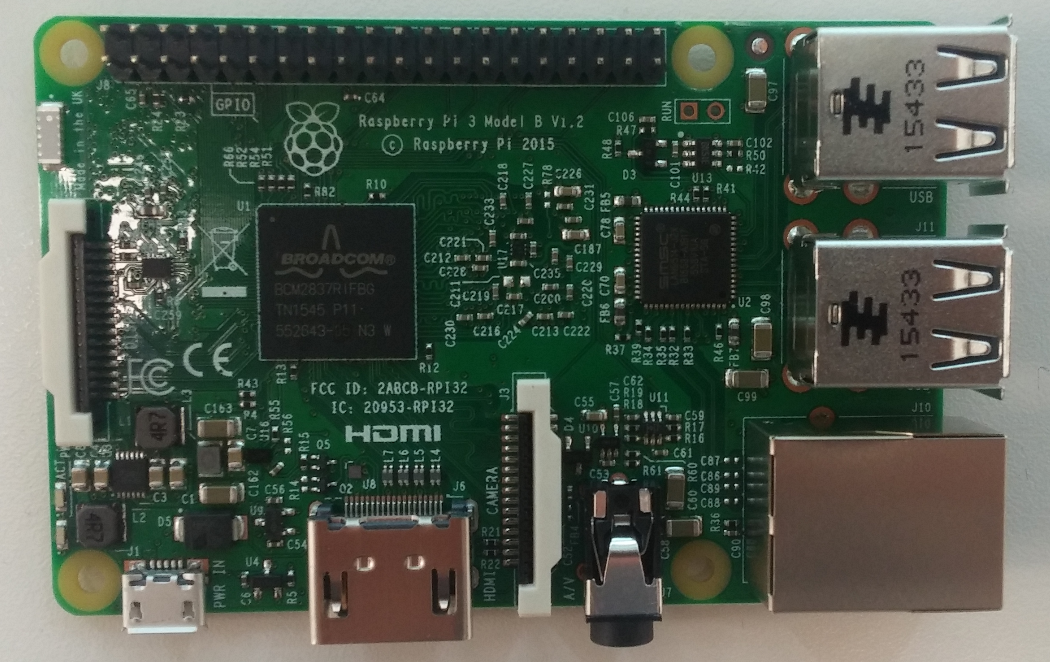
\includegraphics[scale=0.35]{pi3.png}    \caption{Raspberry Pi 3}
    \label{fig:adxl345}
\end{figure}

\begin{figure}[h]
    \centering
    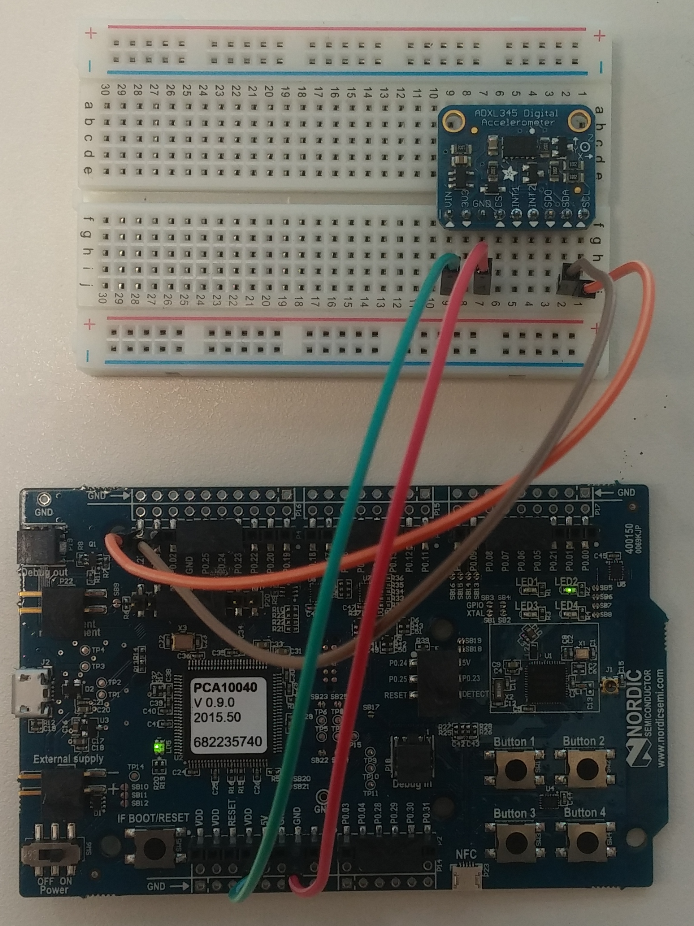
\includegraphics[scale=0.35]{nrf-adxl.png}    \caption{Connected nRF52 -- ADXL345}
    \label{fig:adxl345}
\end{figure}


\section{\gls{6lowpan} and \gls{ble}}



\section{Connecting Raspberry Pi and nRF52}



As a microcontroller the nRF52 works great, both as a low-power and powerful device. 

To set up the communication between these two, the two code examples TWI and Observable server from Nordic was used as a starting point. 


\subsection{\gls{spi}}



\subsection{\gls{i2c}}


\subsection{Problems}




